\documentclass[11pt, letterpaper]{article}

\usepackage[english]{babel}
\usepackage[utf8x]{inputenc}
\usepackage[gen]{eurosym}
\usepackage{amsmath}
\usepackage{amssymb}
\usepackage[dvipsnames]{xcolor}
\usepackage{graphicx}
\usepackage[stable]{footmisc}
\usepackage{caption}
\usepackage{subcaption} 
\usepackage[title]{appendix}

\captionsetup{font=footnotesize}


 
\title{Cap-and-trade Model for the Chilean Energy Market}
\author{P\'ia Amigo, Sebasti\'an Cea, Felipe Feijoo}
\date{\today}

\begin{document}
\maketitle

\section{Mathematical Formulation of the Model}\label{model}

Let us consider a market of $i$ producers, each of them minimizing the cost of operation and investment. We will assume perfect competition among the producers. Our model will assume two basic stages: operation at present (with investment for the future) and the future, at the spot market and trading of emission allowances

\smallskip

At first stage, we consider the current operating plant and the cost of the operation $C_i$, and the quantity produce $Q_i$. The maximum quantity of production at current stage (initial) is $\bar{Q}$. Each producer is allow to emit a certain amount of carbon $A_i$. We consider an auctioneer as the agent selling the allowances and obtaining a revenue for them. The revenue recipients are generally consumers (households) or low-emission companies. The auctioneer will try to maximize this revenue. At this stage, the producer decides the amount $x$ of capacity expansion at a cost $I$ for the uncertain future.
\smallskip

At second stage, in the uncertain future, the producer wants to operate in the most efficient way at the spot market. In addition,  we will consider the existence of a permit trading market, where producers can purchase permits from other producers if they need to surpass the emission allowances, or sell the unused permits if their emissions are below allowances. The producer will evaluate the cost of the uncertain future as risk neutral agents, i.e., as an expectation value and we will assume that the probability is a physical probability, which may be obtained from real world data.
\smallskip

We have described the model considering two stages as a simplification of the problem, but the analysis could be extended to a multistage problem. The variable that accounts for the time periods is $\tau$ (see below).
\smallskip


\begin{figure}[ht!]
 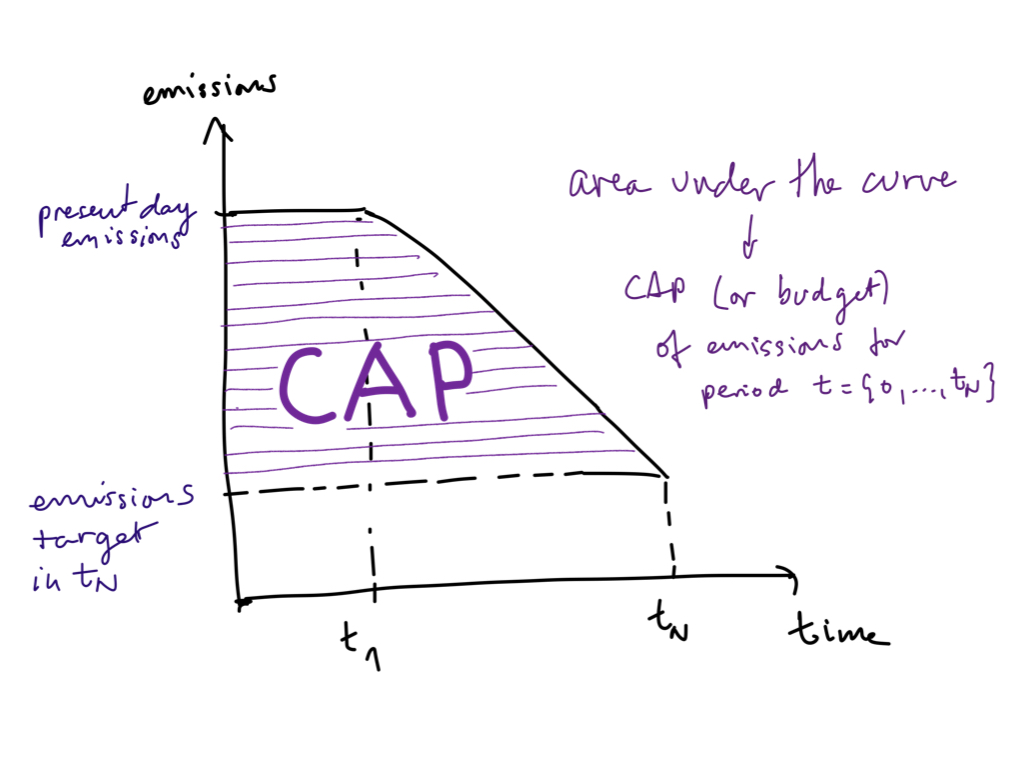
\includegraphics[width=\textwidth]{Informe/cap_scheme.jpeg}
 
 \caption{In a fix period of time, the total amount of carbon emissions allowed by a regulatory agent is CAP, that is, the area under the curve of the plot shown. The allowances sold to the different producers depend on each year, and the shape of the curve might vary, but the CAP, or maximum budget of emissions is fixed. }
 \label{cap-scheme}
\end{figure}

The maximum budget for emissions is the  parameter CAP, which in turn, follows a normal distribution, i.e., $CAP \thicksim N(\mu, \sigma^2)$. This CAP is determined by a regulatory agent and  accounts for the total emissions throughout the whole period considered, that is, does not depend of $\tau$. Figure \ref{cap-scheme} shows a simple scheme of CAP. In a period of years $\tau$, the emissions must be reduced in a certain amount to meet the target. For instance, Chile abides the Paris Agreement and is committed to reduce its emissions to 30\% below its 2007 levels by 2030\footnote{See https://climateactiontracker.org/countries/chile/ for a complete description of Chile's commitment in the Paris Agreement. Still, the promises made are categorized as highly insufficient to hold global warming below 2$^o$. }.

\smallskip
The amount of total allowances provided by the auctioneer $\theta$ is an endogenous random variable in our model, and it must satisfied the condition $\sum_i A_i = \theta$. 
Since $\theta$ must not surpass the budget for emissions, we consider a low margin (or risk) $R$ for this to happen, i.e.,
\begin{equation}
    P (\theta \geq CAP) \leq R
\end{equation}

and since the variable CAP follows a normal distribution with mean $\mu$ and variance $\sigma^2$, we can write the equation above as
\begin{equation}
    \theta \leq \phi^{-1}(R) \sigma^2 + \mu
\end{equation}

where $\phi^{-1}$ is the inverse of the cumulative function of the normal distribution. 

Our model considers the case of incomplete markets. One way to include market incompleteness in our model is to consider some structure for the $V_i$ and $P_i$ variables, as a function of $x$. 




\hspace{0.5cm}

\begin{flushleft}
\textbf{Sets}
\begin{itemize}
    \item[] $i$: number of producers
    \item[] $\omega$: possible scenarios
    \item[] $\tau$: model periods
    
\end{itemize}

\hspace{0.5cm}

\textbf{Parameters}
\begin{itemize}
   \item[] $\bar{Q}_i$: maximum operation capacity
   \item[] $I$: expansion cost
   \item[] $C_i$: operation cost
   \item[] $D$: total demand (exogenous)
   \item[] $CAP$: maximum budget of emissions 
   \item[] $R$: margin for total emission allowances
 \item[] $\varepsilon_{i}$: Emissions factor of producer $i$
\end{itemize}
\hspace{0.5cm}

\textbf{Variables}
\begin{itemize}
    \item[] $Q^{\tau}_i$: produced quantity
    \item[] $A_i$: emission allowances
    \item[] $P^{\tau}_i$: purchased permits
    \item[] $V^{\tau}_i$: sold permits
    \item[] $\lambda$: dual to CAP constraint
    \item[] $\mu$: dual to trading equilibrium
    \item[] $x_i$: capacity expansion decision
    \item[] $\theta_{\omega}$: emission permits available in the market
    \end{itemize}

\hspace{0.5cm}

\textbf{Equations}
\smallskip

Each producer $i$ minimizes cost:
\begin{align}
    \min_{ x,Q,A,P,V} & \sum_{j}C_{i,j} Q^{1}_{i,j} + A_i\lambda^{1}_i + \sum_{j}I_{i,j}x_{i,j} \nonumber \\
     &\qquad - \sum_{\tau > 1} \sum_{\Omega}prob_\omega[\sum_j C_{i,j} Q^{\tau}_{i,j,\omega}  - (V^{\tau}_{i,\omega}-P^{\tau}_{i,\omega})\mu^{\tau}_{i,\omega}]\\
 \textrm{s.t \ } \nonumber
 \end{align}
 \begin{align}
    Q_{i,\omega}^{\tau} & \leq \bar{Q_i} + x_i & \forall & \quad \omega, \tau  > 1 & \quad (\alpha_{i,\omega,\tau})\\
    Q_{i}^{\tau} & \leq \bar{Q_i}  &  & \quad \tau  =1 & \quad (\kappa_i) \\
 A_{i} + P_{i,\omega} & \geq  V_{i,\omega} & \forall & \quad \omega & \quad (\beta_{i,\omega})\\
 \sum_{\tau>1}Q_{i, \omega}^{\tau}\varepsilon_{i} & \leq  A_{i} + P_{i,\omega} - V_{i,\omega}  &\forall & \quad \omega & \quad (\gamma_{i,\omega})\\
 Q_{i, \omega}^{\tau} & \geq  0   & \forall & \quad \omega, \tau & \quad (\delta_{i,\omega})
\end{align}

\smallskip
Auctioneer:
\begin{align}
    \max_{\theta} & \ \theta \lambda \\
    \textrm{s.t \ } & P(\theta \geq CAP) \leq R\\
    & \theta \geq 0
\end{align}

\smallskip

\textbf{Market clearing constraints}

\begin{align}
\textrm{(available allowances)}: &  \ \   \sum_{\tau} \sum_{i} A^{\tau}_{i,\omega} = \theta   & \forall \ \omega & \ \  (\lambda)\\
\textrm{(equilibrium in trading market)}: &   \ \  \sum_{i} P^{\tau}_{i,\omega} = \sum_{i} V^{\tau}_{i,\omega} & \forall \ \omega, \tau & \ \ (\mu) \\
\textrm{(fulfillment of the demand)}:  &   \ \  \sum_{i,j} Q^{\tau}_{i, j,\omega} = D^{\tau}_{\omega}, & \forall \ \omega, \tau & \ \ (\pi)
\end{align}

\end{flushleft}


\section{KKT conditions}
We will start by considering the simplest case of our model, that is two producers, each one only producing one technology. The analysis is performed as two stages. The market is complete, i.e., there is no constraint in the sold or purchase amount of emission permits ($V_{i,\omega}$ and  $P_{i,\omega}$ respectively). The model below is defined for each $i \in \{ 1,...,n\}$

\begin{align}
    \min_{x,Q,A,P,V} & C_iQ_i^{1} + A_i \lambda + I_i x_i + \sum_{\Omega} prob_\omega \Big[ \sum_{\tau>1} (C_i-\pi_{\omega}) Q_{i,\omega}^{\tau}-(V_{i,\omega}-P_{i,\omega})\mu_{\omega}\Big]\\
     \textrm{s.t \ } \nonumber
\end{align}
\begin{align}
    Q_{i,\omega}^{\tau} & \leq \bar{Q_i} + x_i & \forall & \quad \omega, \tau  > 1 & \quad (\alpha_{i,\omega,\tau})\\
    Q_{i}^{\tau} & \leq \bar{Q_i}  &  & \quad \tau  =1 & \quad (\kappa_i) \\
 A_{i} + P_{i,\omega} & \geq  V_{i,\omega} & \forall & \quad \omega & \quad (\beta_{i,\omega})\\
 \sum_{\tau>1}Q_{i, \omega}^{\tau}\varepsilon_{i} & \leq  A_{i} + P_{i,\omega} - V_{i,\omega}  &\forall & \quad \omega & \quad (\gamma_{i,\omega})\\
 Q_{i, \omega}^{\tau} & \geq  0   & \forall & \quad \omega, \tau & \quad (\delta_{i,\omega})
\end{align}

The Lagrangian function for each $i \in \{ 1,...,n\}$ is defined as follows:

\begin{multline}
    \mathcal{L}_i(x,Q,A,P,V) = C_i Q_i^{1} + A_i \lambda + I_i x_i \\
    + \sum_{\Omega} prob_\omega \Big[(C_i-\pi_{\omega}) Q_{i,\omega}^{\tau} - (V_{i,\omega} - P_{i,\omega}) \mu_{\omega}\Big]+ \kappa_{i}\Big[Q_{i}^{1} - \bar{Q_i}\Big] +\sum_{\omega,\tau>1} \alpha_{i,\omega,\tau}\Big[Q_{i,\omega}^{\tau} - (\bar{Q_i}+ x_i)\Big] \\ + \sum_{\omega}\beta_{i,\omega}\Big[V_{i,\omega}-(A_i + P_{i,\omega})\Big] + \sum_{\omega}\gamma_{i,\omega} \Big[\sum_{\tau>1}Q_{i,\omega}^{\tau} \varepsilon_{i} - (A_i + P_{i,\omega} -V_{i,\omega})\Big] + \sum_{\omega, \tau>1}\delta_{i,\omega,\tau} \Big[0-Q_{i,\omega}^{\tau}\Big] + \eta_{i}\Big[0-Q^{1}_{i}\Big]
\end{multline}

where $\alpha_{i,\omega,\tau}$, $\kappa_i$, $\beta_{i,\omega}$, $\gamma_{i,\omega}$ and $\delta_{i,\omega}$ are the lagrange multipliers of the constraints. 

With the Lagrangian set up, we can now find de KKT conditions for each of the producers $i \in \{ 1,...,n\}$ by making $\nabla \mathcal{L}_{i}=0$, we obtain:

\begin{align}
    I_i - \sum_{\omega,\tau>1} \alpha_{i,\omega,\tau} & = 0 & \forall i  &  \qquad (x_i)\\
    C_{i} + \kappa - \eta_{i} & = 0 & \forall i  &  \qquad (Q^{1}_{i})\\
    prob_\omega (C_i-\pi_{\omega}) + \alpha_{\omega,\tau} + \gamma_{i,\omega} \varepsilon_{i}-\delta_{\omega,\tau} & =0 & \forall i, \omega, \tau>1 &  \qquad (Q_{i,\omega}^{\tau})\\
    \lambda - \sum_{\omega}\beta_{i,\omega} - \sum_{\omega}\gamma_{i,\omega} & =0 & \forall i & \qquad (A_{i}) \\
    prob_\omega \mu_{\omega} - \beta_{i,\omega}  - \gamma_{i,\omega} & =0 & \forall i, \omega & \qquad (V_{i,\omega}) \\
    prob_\omega \mu_{\omega} - \beta_{i,\omega} -\gamma_{i,\omega} & = 0 & \forall i, \omega & \qquad (P_{i,\omega})
\end{align}

\smallskip


\begin{flushleft}
Primal feasibility
\end{flushleft}

\begin{align}
    -Q_{i,\omega}^{\tau} + \bar{Q_i} + x_i & \geq 0 & \qquad (\alpha_{i,\omega,\tau}) \\
    -\bar{Q_i} + Q^{\tau}_i & \geq 0 & \qquad (\kappa_i)\\
     A_{i} + P_{i,\omega} - V_{i,\omega} & \geq 0 & \qquad (\beta_{i,\omega}) \\
     A_{i} + P_{i,\omega} - V_{i,\omega} - \sum_{\tau>1}Q_{i, \omega}^{\tau}\varepsilon_{i} & \geq 0 & \qquad (\gamma_{i,\omega}) \\
    Q_{i,\omega}^{\tau} & \geq 0 & \qquad (\delta_{i,\omega})
\end{align}

\smallskip

\begin{flushleft}
Complementary slackness\\

\textbf{FALTAN los For all i,w,t...etc}
\end{flushleft}

\begin{align}
    (-Q_{i,\omega}^{\tau} + \bar{Q_i} + x_i)\alpha_{i,\omega,\tau} & = 0 \\
    ( -\bar{Q_i} + Q^{\tau}_i)\kappa_i & = 0 \\
    (V_{i,\omega} - A_{i} - P_{i,\omega})\beta_{i,\omega} & = 0 \\
    ( A_{i} + P_{i,\omega} - V_{i,\omega} - \sum_{\tau>1}Q_{i, \omega}^{\tau}\varepsilon_{i})\gamma_{i,\omega} & = 0 \\
    Q_{i,\omega}^{\tau}\delta_{i,\omega} & = 0
\end{align}

\smallskip

\begin{flushleft}
Dual Feasibility
\end{flushleft}

\begin{align}
    \alpha_{i,\omega,\tau} & \geq 0 \\
    \kappa_i & \geq 0 \\
    \beta_{i,\omega} & \geq 0 \\
    \gamma_{i,\omega} & \geq 0 \\
    \delta_{i,\omega} & \geq 0 
\end{align}

Now we consider the Auctioneer agent, which regulates the amount of permits allowed in the market.
The auctioner must maximizes revenue from permits, but we will write as a minimization problem:

\begin{align}
    \min_{\theta} & -\theta \lambda \\
    \textrm{s.t \ } & \theta \leq \phi^{-1}(R) \sigma^2 + \mu \\
    &\theta \geq 0
\end{align}

For the Auctioneer, the Lagrangian function is 

\begin{equation}
    \mathcal{L}(\theta)= -\theta \lambda + \eta (\theta - \phi^{-1}(R) \sigma^2 - \mu ) + dt(0-\theta)
\end{equation}

where $\eta$ is the lagrange multiplier. Thus, we can obtain the KKT conditions for the auctioneer problem.

\begin{align}
    -\lambda +\eta -dt & = 0 \\
    \theta & \geq  0 \\
    (\theta - \phi^{-1}(R) \sigma^2 - \mu) \eta & =  0\\
    \eta & \geq  0
\end{align}

\end{document}